\documentclass[oneside]{memoir}
\usepackage{fontspec}
\usepackage[hidelinks]{hyperref}
\usepackage{microtype}
\usepackage{amsmath}
\usepackage{amssymb}
\usepackage{bm}
\usepackage{xcolor}
\usepackage{booktabs}
\usepackage{graphicx}
\usepackage[euler-digits,euler-hat-accent]{eulervm}

\setlrmarginsandblock{3.5cm}{2.5cm}{*}
\setulmarginsandblock{2.5cm}{*}{1}
\checkandfixthelayout

\definecolor{ACCgreen}{HTML}{28A745}

\newcommand\ddfrac[2]{\frac{\displaystyle #1}{\displaystyle #2}}

\setmainfont{TeX Gyre Pagella}

\usepackage{xcolor}
\hypersetup{
    colorlinks,
    linkcolor={red!50!black},
    citecolor={blue!50!black},
    urlcolor={blue!80!black}
}

\def\chapterheadstart{}
\pagestyle{empty}

\begin{document}

\begin{figure}
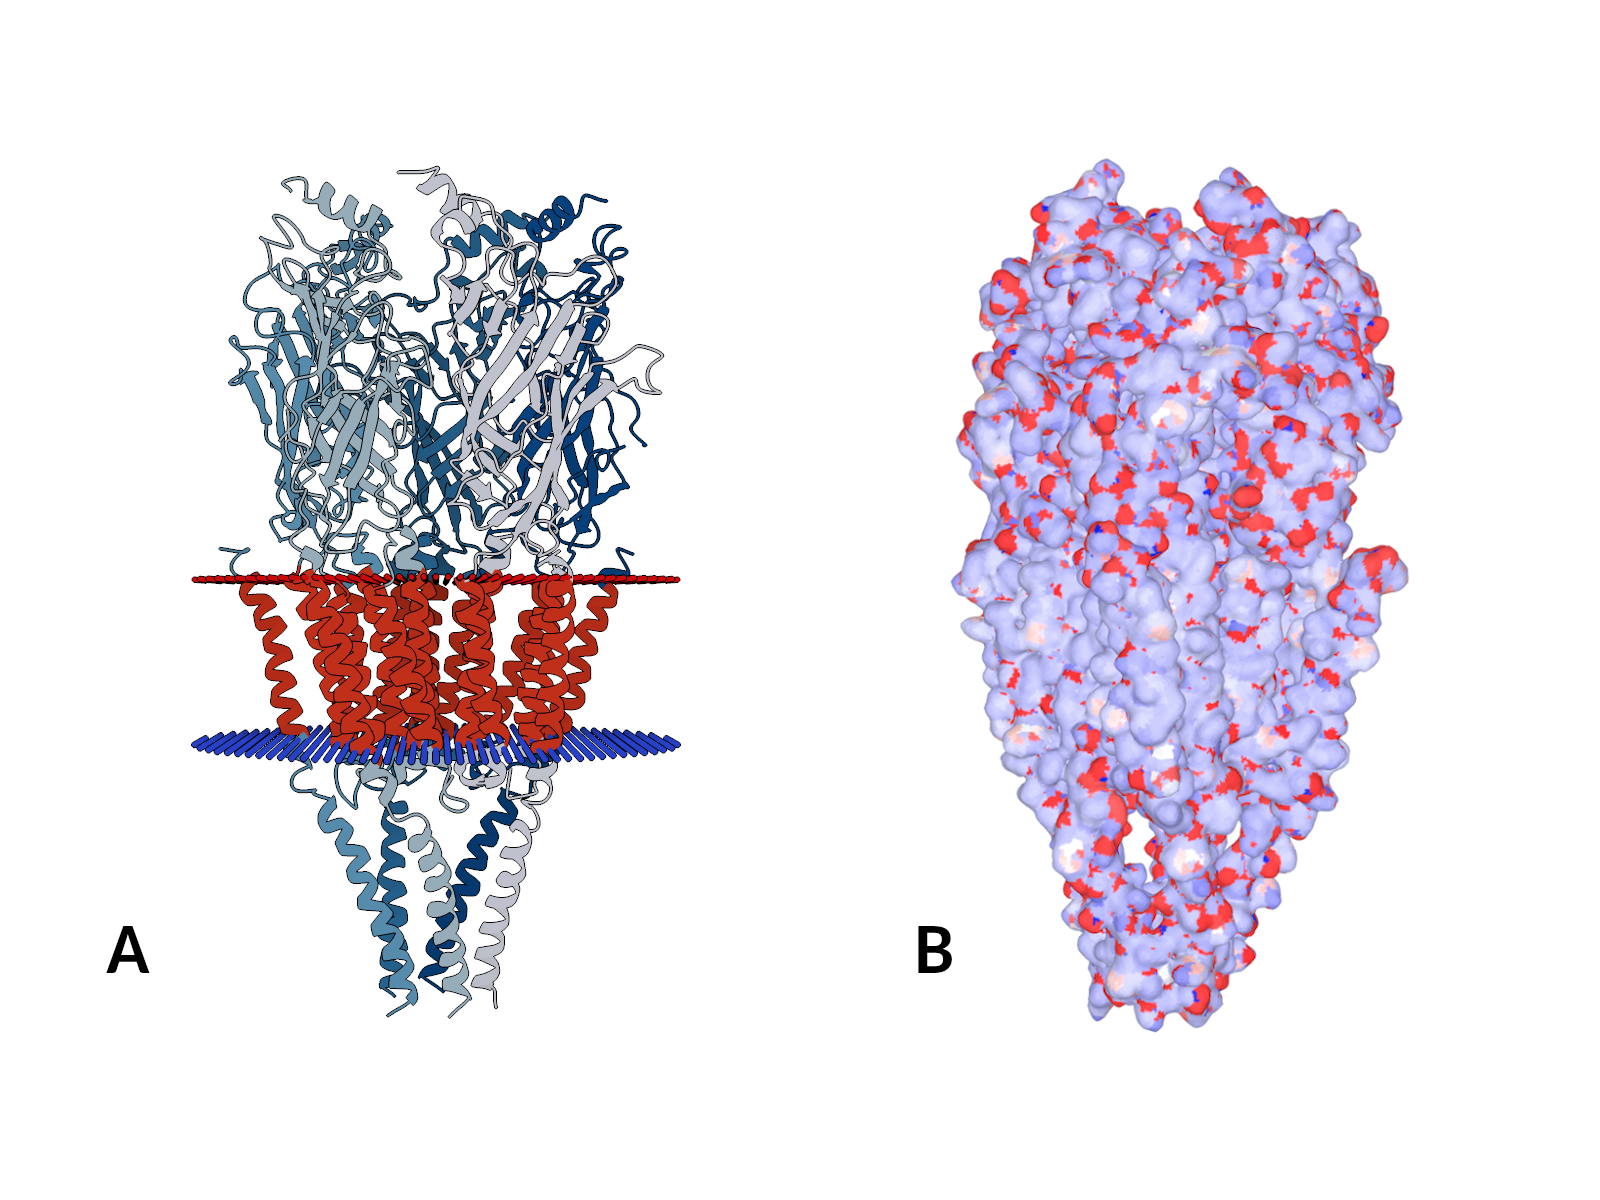
\includegraphics[width=.9\linewidth]{figure4.png}
\renewcommand{\thefigure}{4}
\caption{A structure of nicotinic acetylcholine receptor (PDB ID \href{https://www.ebi.ac.uk/pdbe/entry/pdb/2bg9}{2bg9}): A) A scheme showing the receptor (in grey) passing the membrane (in red). The figure was overtaken from RCSB PDB. B) Partial atomic charges (from ACC II) visualized on the surface of the receptor structure showing distinct areas: Nonpolar transmembrane part (mostly white due to charge around zero) and polar surface of extracellular and cytoplasmic parts (with a mosaic of blue positive and red negative charges).}
\end{figure}

\end{document} 


